\documentclass[12pt]{article}
\usepackage{amsmath}
\usepackage{graphicx}
\usepackage[margin=0.9in]{geometry}
\setlength{\emergencystretch}{2em}
\begin{document}
\title{RoMMath Origin Items with Adversarial Variants}
\author{}
\date{}
\maketitle
\section*{geo1021-origin}
\noindent\begin{minipage}{\textwidth}
\setlength{\parskip}{4pt}
As shown in the figure, given that the equilateral triangle \ensuremath{\triangle }ABC has BC as the diameter of the circle intersecting AB at D and AC at E, if BC=2, then what is the length of CD?\\
Instructions:\\
- Do NOT assume figures are to scale.\\
- Use ONLY marks visible in the diagram unless explicitly stated in the text.\\
- Follow the output contract below exactly.\\
\end{minipage}
\begin{center}
\begin{minipage}{0.32\textwidth}\centering
Base\\
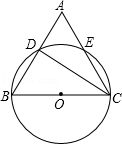
\includegraphics[width=0.95\linewidth]{out_rommath_origin/items/geo1021-origin/assets/figure.png}
\end{minipage}
\par
\end{center}
\bigskip
\section*{geo1025-origin}
\noindent\begin{minipage}{\textwidth}
\setlength{\parskip}{4pt}
As shown in the figure, points A, E, and B are on circle O. The inscribed angle \ensuremath{\angle }ACE is 25\ensuremath{^\circ}, and \ensuremath{\angle }BDE is 15\ensuremath{^\circ}. What is the measure of the central angle \ensuremath{\angle }AOB?\\
Instructions:\\
- Do NOT assume figures are to scale.\\
- Use ONLY marks visible in the diagram unless explicitly stated in the text.\\
- Follow the output contract below exactly.\\
\end{minipage}
\begin{center}
\begin{minipage}{0.32\textwidth}\centering
Base\\
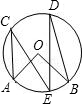
\includegraphics[width=0.95\linewidth]{out_rommath_origin/items/geo1025-origin/assets/figure.png}
\end{minipage}
\par
\end{center}
\bigskip
\section*{geo1045-origin}
\noindent\begin{minipage}{\textwidth}
\setlength{\parskip}{4pt}
As shown in the figure, PA is the tangent to circle O at point A, PO=2, and \ensuremath{\angle }APO=30\ensuremath{^\circ}. What is the length of PA?\\
Instructions:\\
- Do NOT assume figures are to scale.\\
- Use ONLY marks visible in the diagram unless explicitly stated in the text.\\
- Follow the output contract below exactly.\\
\end{minipage}
\begin{center}
\begin{minipage}{0.32\textwidth}\centering
Base\\
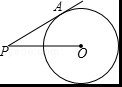
\includegraphics[width=0.95\linewidth]{out_rommath_origin/items/geo1045-origin/assets/figure.png}
\end{minipage}
\par
\end{center}
\bigskip
\section*{geo137-origin}
\noindent\begin{minipage}{\textwidth}
\setlength{\parskip}{4pt}
If P R \textbackslash{}parallel W X, W X = 10, X Y = 6, W Y = 8, R Y = 5, and P S = 3, find P Y.\\
Instructions:\\
- Do NOT assume figures are to scale.\\
- Use ONLY marks visible in the diagram unless explicitly stated in the text.\\
- Follow the output contract below exactly.\\
\end{minipage}
\begin{center}
\begin{minipage}{0.32\textwidth}\centering
Base\\
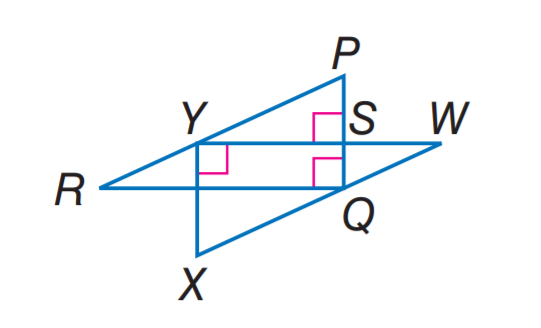
\includegraphics[width=0.95\linewidth]{out_rommath_origin/items/geo137-origin/assets/figure.png}
\end{minipage}
\hfill\begin{minipage}{0.32\textwidth}\centering
geo137-origin\_rot30\\
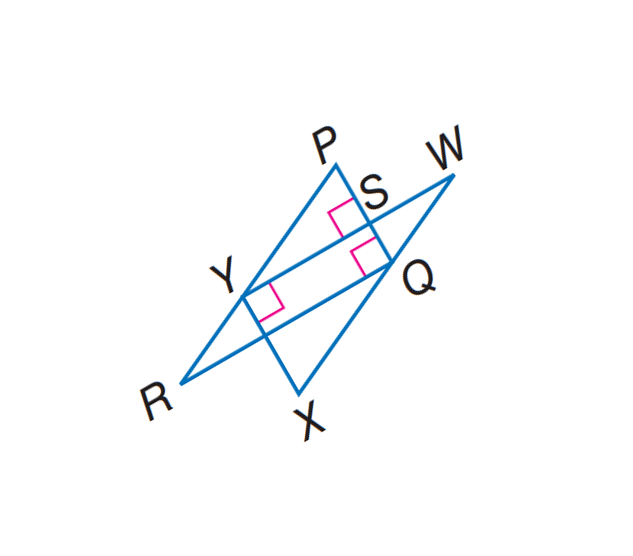
\includegraphics[width=0.95\linewidth]{out_rommath_origin/items/geo137-origin/assets/figure_rot30.png}
\end{minipage}
\hfill\begin{minipage}{0.32\textwidth}\centering
geo137-origin\_rot90\\
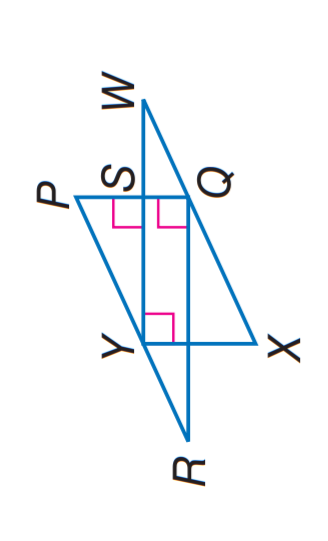
\includegraphics[width=0.95\linewidth]{out_rommath_origin/items/geo137-origin/assets/figure_rot90.png}
\end{minipage}
\par\medskip
\begin{minipage}{0.32\textwidth}\centering
geo137-origin\_rot180\\
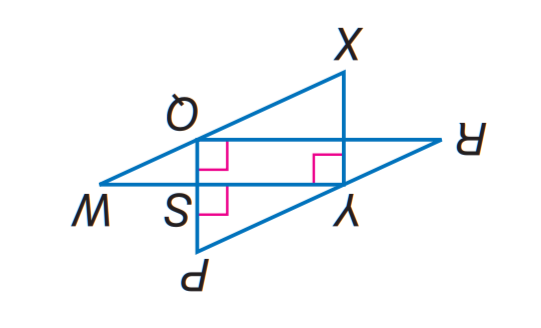
\includegraphics[width=0.95\linewidth]{out_rommath_origin/items/geo137-origin/assets/figure_rot180.png}
\end{minipage}
\hfill\begin{minipage}{0.32\textwidth}\centering
geo137-origin\_circle\_enclose\\
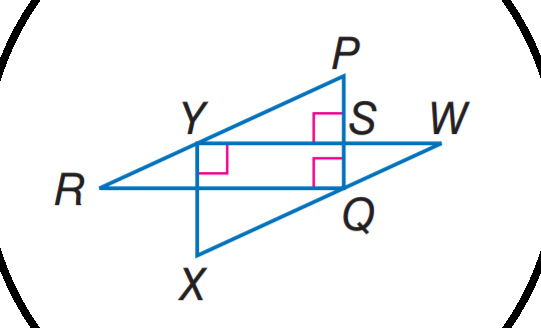
\includegraphics[width=0.95\linewidth]{out_rommath_origin/items/geo137-origin/assets/figure_circle.png}
\end{minipage}
\par
\end{center}
\bigskip
\section*{geo231-origin}
\noindent\begin{minipage}{\textwidth}
\setlength{\parskip}{4pt}
In \textbackslash{}triangle P Q R, Z Q = 3 a - 11, Z P = a + 5, P Y = 2 c - 1, Y R = 4 c - 11, m \textbackslash{}angle P R Z = 4 b - 17, m \textbackslash{}angle Z R Q = 3 b - 4, m \textbackslash{}angle Q Y R = 7 b + 6, and m \textbackslash{}angle P X R = 2 a + 10. If Q Y is a perpendicular bisector of P R, find b.\\
Instructions:\\
- Do NOT assume figures are to scale.\\
- Use ONLY marks visible in the diagram unless explicitly stated in the text.\\
- Follow the output contract below exactly.\\
\end{minipage}
\begin{center}
\begin{minipage}{0.32\textwidth}\centering
Base\\
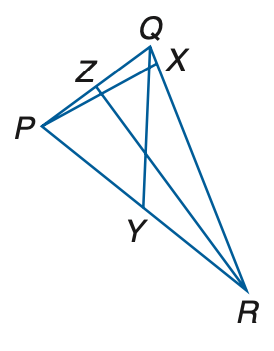
\includegraphics[width=0.95\linewidth]{out_rommath_origin/items/geo231-origin/assets/figure.png}
\end{minipage}
\hfill\begin{minipage}{0.32\textwidth}\centering
geo231-origin\_rot30\\
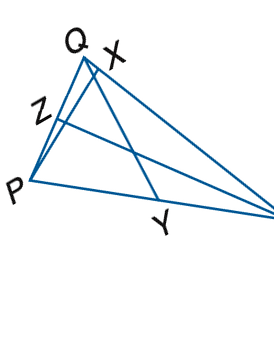
\includegraphics[width=0.95\linewidth]{out_rommath_origin/items/geo231-origin/assets/figure_rot30.png}
\end{minipage}
\hfill\begin{minipage}{0.32\textwidth}\centering
geo231-origin\_rot90\\
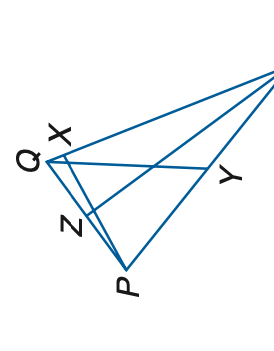
\includegraphics[width=0.95\linewidth]{out_rommath_origin/items/geo231-origin/assets/figure_rot90.png}
\end{minipage}
\par\medskip
\begin{minipage}{0.32\textwidth}\centering
geo231-origin\_rot180\\
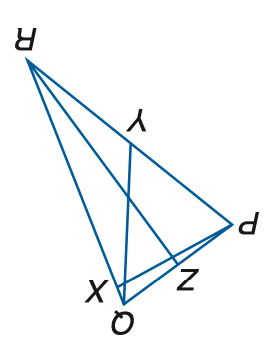
\includegraphics[width=0.95\linewidth]{out_rommath_origin/items/geo231-origin/assets/figure_rot180.png}
\end{minipage}
\hfill\begin{minipage}{0.32\textwidth}\centering
geo231-origin\_circle\_enclose\\
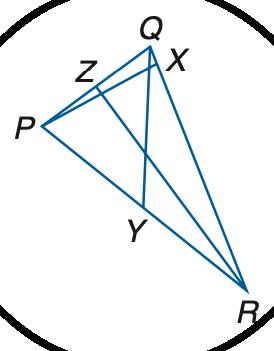
\includegraphics[width=0.95\linewidth]{out_rommath_origin/items/geo231-origin/assets/figure_circle.png}
\end{minipage}
\par
\end{center}
\bigskip
\section*{geo233-origin}
\noindent\begin{minipage}{\textwidth}
\setlength{\parskip}{4pt}
In \textbackslash{}triangle D E F, P is the midpoint of D E, and Q is the midpoint of side D F. If E F = 3 x + 4 and P Q = 20, what is the value of x?\\
Instructions:\\
- Do NOT assume figures are to scale.\\
- Use ONLY marks visible in the diagram unless explicitly stated in the text.\\
- Follow the output contract below exactly.\\
\end{minipage}
\begin{center}
\begin{minipage}{0.32\textwidth}\centering
Base\\
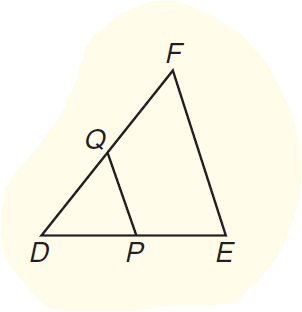
\includegraphics[width=0.95\linewidth]{out_rommath_origin/items/geo233-origin/assets/figure.png}
\end{minipage}
\hfill\begin{minipage}{0.32\textwidth}\centering
geo233-origin\_rot30\\
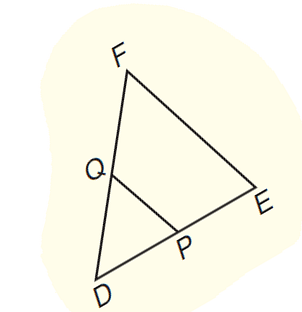
\includegraphics[width=0.95\linewidth]{out_rommath_origin/items/geo233-origin/assets/figure_rot30.png}
\end{minipage}
\hfill\begin{minipage}{0.32\textwidth}\centering
geo233-origin\_rot90\\
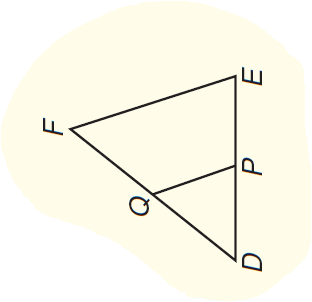
\includegraphics[width=0.95\linewidth]{out_rommath_origin/items/geo233-origin/assets/figure_rot90.png}
\end{minipage}
\par\medskip
\begin{minipage}{0.32\textwidth}\centering
geo233-origin\_rot180\\
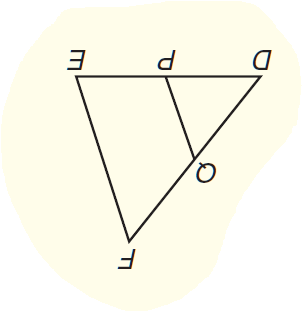
\includegraphics[width=0.95\linewidth]{out_rommath_origin/items/geo233-origin/assets/figure_rot180.png}
\end{minipage}
\hfill\begin{minipage}{0.32\textwidth}\centering
geo233-origin\_circle\_enclose\\
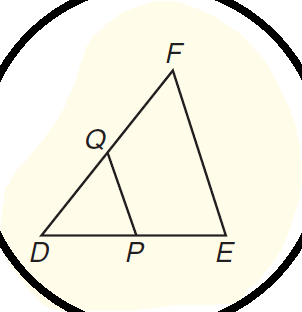
\includegraphics[width=0.95\linewidth]{out_rommath_origin/items/geo233-origin/assets/figure_circle.png}
\end{minipage}
\par
\end{center}
\bigskip
\section*{geo313-origin}
\noindent\begin{minipage}{\textwidth}
\setlength{\parskip}{4pt}
As shown in the figure, in \ensuremath{\triangle }ABC, AC = 4 cm, the perpendicular bisector of segment AB intersects AC at point N, and the perimeter of \ensuremath{\triangle }BCN is 7 cm. What is the length of BC?\\
Instructions:\\
- Do NOT assume figures are to scale.\\
- Use ONLY marks visible in the diagram unless explicitly stated in the text.\\
- Follow the output contract below exactly.\\
\end{minipage}
\begin{center}
\begin{minipage}{0.32\textwidth}\centering
Base\\
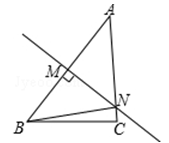
\includegraphics[width=0.95\linewidth]{out_rommath_origin/items/geo313-origin/assets/figure.png}
\end{minipage}
\hfill\begin{minipage}{0.32\textwidth}\centering
geo313-origin\_rot30\\
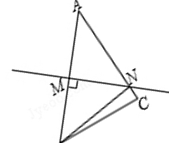
\includegraphics[width=0.95\linewidth]{out_rommath_origin/items/geo313-origin/assets/figure_rot30.png}
\end{minipage}
\hfill\begin{minipage}{0.32\textwidth}\centering
geo313-origin\_rot90\\
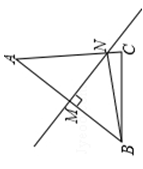
\includegraphics[width=0.95\linewidth]{out_rommath_origin/items/geo313-origin/assets/figure_rot90.png}
\end{minipage}
\par\medskip
\begin{minipage}{0.32\textwidth}\centering
geo313-origin\_rot180\\
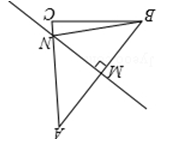
\includegraphics[width=0.95\linewidth]{out_rommath_origin/items/geo313-origin/assets/figure_rot180.png}
\end{minipage}
\hfill\begin{minipage}{0.32\textwidth}\centering
geo313-origin\_circle\_enclose\\
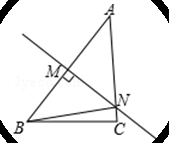
\includegraphics[width=0.95\linewidth]{out_rommath_origin/items/geo313-origin/assets/figure_circle.png}
\end{minipage}
\par
\end{center}
\bigskip
\section*{geo321-origin}
\noindent\begin{minipage}{\textwidth}
\setlength{\parskip}{4pt}
As shown in the figure, AB \ensuremath{\parallel } CD, \ensuremath{\angle }E = 40\ensuremath{^\circ}, \ensuremath{\angle }A = 110\ensuremath{^\circ}, then the degree of \ensuremath{\angle }C is ()\\
Instructions:\\
- Do NOT assume figures are to scale.\\
- Use ONLY marks visible in the diagram unless explicitly stated in the text.\\
- Follow the output contract below exactly.\\
\end{minipage}
\begin{center}
\begin{minipage}{0.32\textwidth}\centering
Base\\
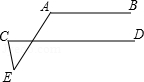
\includegraphics[width=0.95\linewidth]{out_rommath_origin/items/geo321-origin/assets/figure.png}
\end{minipage}
\hfill\begin{minipage}{0.32\textwidth}\centering
geo321-origin\_rot30\\
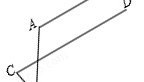
\includegraphics[width=0.95\linewidth]{out_rommath_origin/items/geo321-origin/assets/figure_rot30.png}
\end{minipage}
\hfill\begin{minipage}{0.32\textwidth}\centering
geo321-origin\_rot90\\
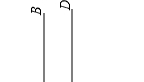
\includegraphics[width=0.95\linewidth]{out_rommath_origin/items/geo321-origin/assets/figure_rot90.png}
\end{minipage}
\par\medskip
\begin{minipage}{0.32\textwidth}\centering
geo321-origin\_rot180\\
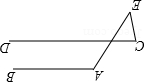
\includegraphics[width=0.95\linewidth]{out_rommath_origin/items/geo321-origin/assets/figure_rot180.png}
\end{minipage}
\hfill\begin{minipage}{0.32\textwidth}\centering
geo321-origin\_circle\_enclose\\
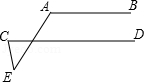
\includegraphics[width=0.95\linewidth]{out_rommath_origin/items/geo321-origin/assets/figure_circle.png}
\end{minipage}
\par
\end{center}
\bigskip
\section*{geo328-origin}
\noindent\begin{minipage}{\textwidth}
\setlength{\parskip}{4pt}
As shown in the figure, AB is the diameter of circle O, and quadrilateral ABCD is an inscribed quadrilateral of circle O. Point P is on the extension of BA, and PD is tangent to circle O at point D. If \ensuremath{\angle }BCD = 120\ensuremath{^\circ}, then what is the measure of \ensuremath{\angle }APD?\\
Instructions:\\
- Do NOT assume figures are to scale.\\
- Use ONLY marks visible in the diagram unless explicitly stated in the text.\\
- Follow the output contract below exactly.\\
\end{minipage}
\begin{center}
\begin{minipage}{0.32\textwidth}\centering
Base\\
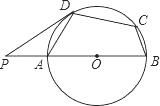
\includegraphics[width=0.95\linewidth]{out_rommath_origin/items/geo328-origin/assets/figure.png}
\end{minipage}
\hfill\begin{minipage}{0.32\textwidth}\centering
geo328-origin\_rot30\\
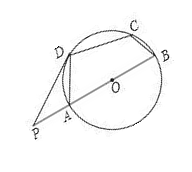
\includegraphics[width=0.95\linewidth]{out_rommath_origin/items/geo328-origin/assets/figure_rot30.png}
\end{minipage}
\hfill\begin{minipage}{0.32\textwidth}\centering
geo328-origin\_rot90\\
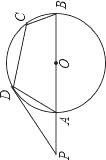
\includegraphics[width=0.95\linewidth]{out_rommath_origin/items/geo328-origin/assets/figure_rot90.png}
\end{minipage}
\par\medskip
\begin{minipage}{0.32\textwidth}\centering
geo328-origin\_rot180\\
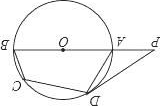
\includegraphics[width=0.95\linewidth]{out_rommath_origin/items/geo328-origin/assets/figure_rot180.png}
\end{minipage}
\hfill\begin{minipage}{0.32\textwidth}\centering
geo328-origin\_circle\_enclose\\
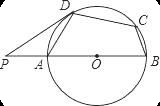
\includegraphics[width=0.95\linewidth]{out_rommath_origin/items/geo328-origin/assets/figure_circle.png}
\end{minipage}
\par
\end{center}
\bigskip
\section*{geo338-origin}
\noindent\begin{minipage}{\textwidth}
\setlength{\parskip}{4pt}
As shown in the figure, AB is tangent to circle O at point A, BO intersects circle O at point C, and point D is on the major arc AC. Given that \ensuremath{\angle }CDA = 27\ensuremath{^\circ}, what is the measure of \ensuremath{\angle }B?\\
Instructions:\\
- Do NOT assume figures are to scale.\\
- Use ONLY marks visible in the diagram unless explicitly stated in the text.\\
- Follow the output contract below exactly.\\
\end{minipage}
\begin{center}
\begin{minipage}{0.32\textwidth}\centering
Base\\
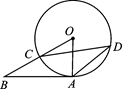
\includegraphics[width=0.95\linewidth]{out_rommath_origin/items/geo338-origin/assets/figure.png}
\end{minipage}
\hfill\begin{minipage}{0.32\textwidth}\centering
geo338-origin\_rot30\\
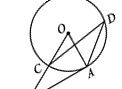
\includegraphics[width=0.95\linewidth]{out_rommath_origin/items/geo338-origin/assets/figure_rot30.png}
\end{minipage}
\hfill\begin{minipage}{0.32\textwidth}\centering
geo338-origin\_rot90\\
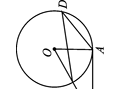
\includegraphics[width=0.95\linewidth]{out_rommath_origin/items/geo338-origin/assets/figure_rot90.png}
\end{minipage}
\par\medskip
\begin{minipage}{0.32\textwidth}\centering
geo338-origin\_rot180\\
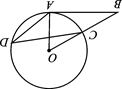
\includegraphics[width=0.95\linewidth]{out_rommath_origin/items/geo338-origin/assets/figure_rot180.png}
\end{minipage}
\hfill\begin{minipage}{0.32\textwidth}\centering
geo338-origin\_circle\_enclose\\
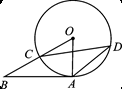
\includegraphics[width=0.95\linewidth]{out_rommath_origin/items/geo338-origin/assets/figure_circle.png}
\end{minipage}
\par
\end{center}
\bigskip
\section*{geo373-origin}
\noindent\begin{minipage}{\textwidth}
\setlength{\parskip}{4pt}
As shown in the figure, the radius of circle O is 5, the chord AB = 5\ensuremath{\sqrt{3}}, and C is a point on the circle. What is the measure of \ensuremath{\angle }ACB?\\
Instructions:\\
- Do NOT assume figures are to scale.\\
- Use ONLY marks visible in the diagram unless explicitly stated in the text.\\
- Follow the output contract below exactly.\\
\end{minipage}
\begin{center}
\begin{minipage}{0.32\textwidth}\centering
Base\\
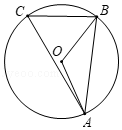
\includegraphics[width=0.95\linewidth]{out_rommath_origin/items/geo373-origin/assets/figure.png}
\end{minipage}
\hfill\begin{minipage}{0.32\textwidth}\centering
geo373-origin\_rot30\\
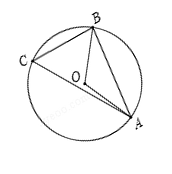
\includegraphics[width=0.95\linewidth]{out_rommath_origin/items/geo373-origin/assets/figure_rot30.png}
\end{minipage}
\hfill\begin{minipage}{0.32\textwidth}\centering
geo373-origin\_rot90\\
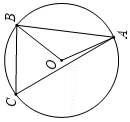
\includegraphics[width=0.95\linewidth]{out_rommath_origin/items/geo373-origin/assets/figure_rot90.png}
\end{minipage}
\par\medskip
\begin{minipage}{0.32\textwidth}\centering
geo373-origin\_rot180\\
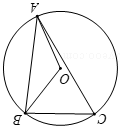
\includegraphics[width=0.95\linewidth]{out_rommath_origin/items/geo373-origin/assets/figure_rot180.png}
\end{minipage}
\hfill\begin{minipage}{0.32\textwidth}\centering
geo373-origin\_circle\_enclose\\
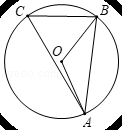
\includegraphics[width=0.95\linewidth]{out_rommath_origin/items/geo373-origin/assets/figure_circle.png}
\end{minipage}
\par
\end{center}
\bigskip
\section*{geo435-origin}
\noindent\begin{minipage}{\textwidth}
\setlength{\parskip}{4pt}
As shown in the figure, point A is on circle O, and BC is a chord of circle O. If \ensuremath{\angle }A = 50\ensuremath{^\circ}, what is the measure of \ensuremath{\angle }OBC?\\
Instructions:\\
- Do NOT assume figures are to scale.\\
- Use ONLY marks visible in the diagram unless explicitly stated in the text.\\
- Follow the output contract below exactly.\\
\end{minipage}
\begin{center}
\begin{minipage}{0.32\textwidth}\centering
Base\\
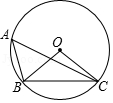
\includegraphics[width=0.95\linewidth]{out_rommath_origin/items/geo435-origin/assets/figure.png}
\end{minipage}
\hfill\begin{minipage}{0.32\textwidth}\centering
geo435-origin\_rot30\\
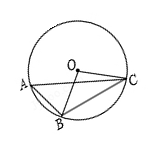
\includegraphics[width=0.95\linewidth]{out_rommath_origin/items/geo435-origin/assets/figure_rot30.png}
\end{minipage}
\hfill\begin{minipage}{0.32\textwidth}\centering
geo435-origin\_rot90\\
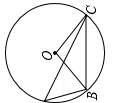
\includegraphics[width=0.95\linewidth]{out_rommath_origin/items/geo435-origin/assets/figure_rot90.png}
\end{minipage}
\par\medskip
\begin{minipage}{0.32\textwidth}\centering
geo435-origin\_rot180\\
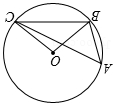
\includegraphics[width=0.95\linewidth]{out_rommath_origin/items/geo435-origin/assets/figure_rot180.png}
\end{minipage}
\hfill\begin{minipage}{0.32\textwidth}\centering
geo435-origin\_circle\_enclose\\
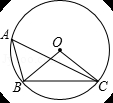
\includegraphics[width=0.95\linewidth]{out_rommath_origin/items/geo435-origin/assets/figure_circle.png}
\end{minipage}
\par
\end{center}
\bigskip
\section*{geo485-origin}
\noindent\begin{minipage}{\textwidth}
\setlength{\parskip}{4pt}
As shown in the figure, AB is the diameter of the semicircle \ensuremath{\odot }O. The sides AC and BC of \ensuremath{\triangle }ABC intersect the semicircle at D and E respectively, and E is the midpoint of BC. Given that \ensuremath{\angle }BAC = 50\ensuremath{^\circ}, find \ensuremath{\angle }C.\\
Instructions:\\
- Do NOT assume figures are to scale.\\
- Use ONLY marks visible in the diagram unless explicitly stated in the text.\\
- Follow the output contract below exactly.\\
\end{minipage}
\begin{center}
\begin{minipage}{0.32\textwidth}\centering
Base\\
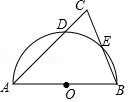
\includegraphics[width=0.95\linewidth]{out_rommath_origin/items/geo485-origin/assets/figure.png}
\end{minipage}
\hfill\begin{minipage}{0.32\textwidth}\centering
geo485-origin\_rot30\\
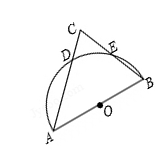
\includegraphics[width=0.95\linewidth]{out_rommath_origin/items/geo485-origin/assets/figure_rot30.png}
\end{minipage}
\hfill\begin{minipage}{0.32\textwidth}\centering
geo485-origin\_rot90\\
\includegraphics[width=0.95\linewidth]{out_rommath_origin/items/geo485-origin/assets/figure_rot90.png}
\end{minipage}
\par\medskip
\begin{minipage}{0.32\textwidth}\centering
geo485-origin\_rot180\\
\includegraphics[width=0.95\linewidth]{out_rommath_origin/items/geo485-origin/assets/figure_rot180.png}
\end{minipage}
\hfill\begin{minipage}{0.32\textwidth}\centering
geo485-origin\_circle\_enclose\\
\includegraphics[width=0.95\linewidth]{out_rommath_origin/items/geo485-origin/assets/figure_circle.png}
\end{minipage}
\par
\end{center}
\bigskip
\section*{geo489-origin}
\noindent\begin{minipage}{\textwidth}
\setlength{\parskip}{4pt}
As shown in the figure, the central angle \ensuremath{\angle }AOB = 60\ensuremath{^\circ}, then the measure of the inscribed angle \ensuremath{\angle }ACB is ()\\
Instructions:\\
- Do NOT assume figures are to scale.\\
- Use ONLY marks visible in the diagram unless explicitly stated in the text.\\
- Follow the output contract below exactly.\\
\end{minipage}
\begin{center}
\begin{minipage}{0.32\textwidth}\centering
Base\\
\includegraphics[width=0.95\linewidth]{out_rommath_origin/items/geo489-origin/assets/figure.png}
\end{minipage}
\hfill\begin{minipage}{0.32\textwidth}\centering
geo489-origin\_rot30\\
\includegraphics[width=0.95\linewidth]{out_rommath_origin/items/geo489-origin/assets/figure_rot30.png}
\end{minipage}
\hfill\begin{minipage}{0.32\textwidth}\centering
geo489-origin\_rot90\\
\includegraphics[width=0.95\linewidth]{out_rommath_origin/items/geo489-origin/assets/figure_rot90.png}
\end{minipage}
\par\medskip
\begin{minipage}{0.32\textwidth}\centering
geo489-origin\_rot180\\
\includegraphics[width=0.95\linewidth]{out_rommath_origin/items/geo489-origin/assets/figure_rot180.png}
\end{minipage}
\hfill\begin{minipage}{0.32\textwidth}\centering
geo489-origin\_circle\_enclose\\
\includegraphics[width=0.95\linewidth]{out_rommath_origin/items/geo489-origin/assets/figure_circle.png}
\end{minipage}
\par
\end{center}
\bigskip
\section*{geo492-origin}
\noindent\begin{minipage}{\textwidth}
\setlength{\parskip}{4pt}
As shown in the figure, in circle O, arc AB is equal to arc BC, point D is on circle O, and angle CDB is 20\ensuremath{^\circ}. What is the measure of angle AOB?\\
Instructions:\\
- Do NOT assume figures are to scale.\\
- Use ONLY marks visible in the diagram unless explicitly stated in the text.\\
- Follow the output contract below exactly.\\
\end{minipage}
\begin{center}
\begin{minipage}{0.32\textwidth}\centering
Base\\
\includegraphics[width=0.95\linewidth]{out_rommath_origin/items/geo492-origin/assets/figure.png}
\end{minipage}
\hfill\begin{minipage}{0.32\textwidth}\centering
geo492-origin\_rot30\\
\includegraphics[width=0.95\linewidth]{out_rommath_origin/items/geo492-origin/assets/figure_rot30.png}
\end{minipage}
\hfill\begin{minipage}{0.32\textwidth}\centering
geo492-origin\_rot90\\
\includegraphics[width=0.95\linewidth]{out_rommath_origin/items/geo492-origin/assets/figure_rot90.png}
\end{minipage}
\par\medskip
\begin{minipage}{0.32\textwidth}\centering
geo492-origin\_rot180\\
\includegraphics[width=0.95\linewidth]{out_rommath_origin/items/geo492-origin/assets/figure_rot180.png}
\end{minipage}
\hfill\begin{minipage}{0.32\textwidth}\centering
geo492-origin\_circle\_enclose\\
\includegraphics[width=0.95\linewidth]{out_rommath_origin/items/geo492-origin/assets/figure_circle.png}
\end{minipage}
\par
\end{center}
\bigskip
\section*{geo500-origin}
\noindent\begin{minipage}{\textwidth}
\setlength{\parskip}{4pt}
As shown in the figure, in circle O, arc AB = arc AC, \ensuremath{\angle }C = 75\ensuremath{^\circ}, then the degree of \ensuremath{\angle }A is ()\\
Instructions:\\
- Do NOT assume figures are to scale.\\
- Use ONLY marks visible in the diagram unless explicitly stated in the text.\\
- Follow the output contract below exactly.\\
\end{minipage}
\begin{center}
\begin{minipage}{0.32\textwidth}\centering
Base\\
\includegraphics[width=0.95\linewidth]{out_rommath_origin/items/geo500-origin/assets/figure.png}
\end{minipage}
\hfill\begin{minipage}{0.32\textwidth}\centering
geo500-origin\_rot30\\
\includegraphics[width=0.95\linewidth]{out_rommath_origin/items/geo500-origin/assets/figure_rot30.png}
\end{minipage}
\hfill\begin{minipage}{0.32\textwidth}\centering
geo500-origin\_rot90\\
\includegraphics[width=0.95\linewidth]{out_rommath_origin/items/geo500-origin/assets/figure_rot90.png}
\end{minipage}
\par\medskip
\begin{minipage}{0.32\textwidth}\centering
geo500-origin\_rot180\\
\includegraphics[width=0.95\linewidth]{out_rommath_origin/items/geo500-origin/assets/figure_rot180.png}
\end{minipage}
\hfill\begin{minipage}{0.32\textwidth}\centering
geo500-origin\_circle\_enclose\\
\includegraphics[width=0.95\linewidth]{out_rommath_origin/items/geo500-origin/assets/figure_circle.png}
\end{minipage}
\par
\end{center}
\bigskip
\section*{geo501-origin}
\noindent\begin{minipage}{\textwidth}
\setlength{\parskip}{4pt}
As shown in the figure, in circle O, chord AB is parallel to chord CD. If \ensuremath{\angle }ABC = 30\ensuremath{^\circ}, then \ensuremath{\angle }BOD = ()\\
Instructions:\\
- Do NOT assume figures are to scale.\\
- Use ONLY marks visible in the diagram unless explicitly stated in the text.\\
- Follow the output contract below exactly.\\
\end{minipage}
\begin{center}
\begin{minipage}{0.32\textwidth}\centering
Base\\
\includegraphics[width=0.95\linewidth]{out_rommath_origin/items/geo501-origin/assets/figure.png}
\end{minipage}
\hfill\begin{minipage}{0.32\textwidth}\centering
geo501-origin\_rot30\\
\includegraphics[width=0.95\linewidth]{out_rommath_origin/items/geo501-origin/assets/figure_rot30.png}
\end{minipage}
\hfill\begin{minipage}{0.32\textwidth}\centering
geo501-origin\_rot90\\
\includegraphics[width=0.95\linewidth]{out_rommath_origin/items/geo501-origin/assets/figure_rot90.png}
\end{minipage}
\par\medskip
\begin{minipage}{0.32\textwidth}\centering
geo501-origin\_rot180\\
\includegraphics[width=0.95\linewidth]{out_rommath_origin/items/geo501-origin/assets/figure_rot180.png}
\end{minipage}
\hfill\begin{minipage}{0.32\textwidth}\centering
geo501-origin\_circle\_enclose\\
\includegraphics[width=0.95\linewidth]{out_rommath_origin/items/geo501-origin/assets/figure_circle.png}
\end{minipage}
\par
\end{center}
\bigskip
\section*{geo508-origin}
\noindent\begin{minipage}{\textwidth}
\setlength{\parskip}{4pt}
As shown in the figure, AB is the diameter of circle O, and chord CD is perpendicular to AB at point E. Given that \ensuremath{\angle }CDB = 30\ensuremath{^\circ} and the radius of circle O is 6, what is the length of the distance OE from the center O to chord CD?\\
Instructions:\\
- Do NOT assume figures are to scale.\\
- Use ONLY marks visible in the diagram unless explicitly stated in the text.\\
- Follow the output contract below exactly.\\
\end{minipage}
\begin{center}
\begin{minipage}{0.32\textwidth}\centering
Base\\
\includegraphics[width=0.95\linewidth]{out_rommath_origin/items/geo508-origin/assets/figure.png}
\end{minipage}
\hfill\begin{minipage}{0.32\textwidth}\centering
geo508-origin\_rot30\\
\includegraphics[width=0.95\linewidth]{out_rommath_origin/items/geo508-origin/assets/figure_rot30.png}
\end{minipage}
\hfill\begin{minipage}{0.32\textwidth}\centering
geo508-origin\_rot90\\
\includegraphics[width=0.95\linewidth]{out_rommath_origin/items/geo508-origin/assets/figure_rot90.png}
\end{minipage}
\par\medskip
\begin{minipage}{0.32\textwidth}\centering
geo508-origin\_rot180\\
\includegraphics[width=0.95\linewidth]{out_rommath_origin/items/geo508-origin/assets/figure_rot180.png}
\end{minipage}
\hfill\begin{minipage}{0.32\textwidth}\centering
geo508-origin\_circle\_enclose\\
\includegraphics[width=0.95\linewidth]{out_rommath_origin/items/geo508-origin/assets/figure_circle.png}
\end{minipage}
\par
\end{center}
\bigskip
\section*{geo509-origin}
\noindent\begin{minipage}{\textwidth}
\setlength{\parskip}{4pt}
As shown in the figure, AB is the diameter of circle O, and chord CD is perpendicular to AB. Given that \ensuremath{\angle }CAB = 40\ensuremath{^\circ}, connect BD and OD. What is the sum of \ensuremath{\angle }AOD and \ensuremath{\angle }ABD?\\
Instructions:\\
- Do NOT assume figures are to scale.\\
- Use ONLY marks visible in the diagram unless explicitly stated in the text.\\
- Follow the output contract below exactly.\\
\end{minipage}
\begin{center}
\begin{minipage}{0.32\textwidth}\centering
Base\\
\includegraphics[width=0.95\linewidth]{out_rommath_origin/items/geo509-origin/assets/figure.png}
\end{minipage}
\hfill\begin{minipage}{0.32\textwidth}\centering
geo509-origin\_rot30\\
\includegraphics[width=0.95\linewidth]{out_rommath_origin/items/geo509-origin/assets/figure_rot30.png}
\end{minipage}
\hfill\begin{minipage}{0.32\textwidth}\centering
geo509-origin\_rot90\\
\includegraphics[width=0.95\linewidth]{out_rommath_origin/items/geo509-origin/assets/figure_rot90.png}
\end{minipage}
\par\medskip
\begin{minipage}{0.32\textwidth}\centering
geo509-origin\_rot180\\
\includegraphics[width=0.95\linewidth]{out_rommath_origin/items/geo509-origin/assets/figure_rot180.png}
\end{minipage}
\hfill\begin{minipage}{0.32\textwidth}\centering
geo509-origin\_circle\_enclose\\
\includegraphics[width=0.95\linewidth]{out_rommath_origin/items/geo509-origin/assets/figure_circle.png}
\end{minipage}
\par
\end{center}
\bigskip
\section*{geo557-origin}
\noindent\begin{minipage}{\textwidth}
\setlength{\parskip}{4pt}
As shown in the figure, AB is the diameter of circle O with a radius of 4. P is an arbitrary point on the circle other than A and B. The bisector of \ensuremath{\angle }APB intersects circle O at point C. Connect AC and BC. The line containing the midline of \ensuremath{\triangle }ABC intersects circle O at points E and F. What is the length of EF?\\
Instructions:\\
- Do NOT assume figures are to scale.\\
- Use ONLY marks visible in the diagram unless explicitly stated in the text.\\
- Follow the output contract below exactly.\\
\end{minipage}
\begin{center}
\begin{minipage}{0.32\textwidth}\centering
Base\\
\includegraphics[width=0.95\linewidth]{out_rommath_origin/items/geo557-origin/assets/figure.png}
\end{minipage}
\hfill\begin{minipage}{0.32\textwidth}\centering
geo557-origin\_rot30\\
\includegraphics[width=0.95\linewidth]{out_rommath_origin/items/geo557-origin/assets/figure_rot30.png}
\end{minipage}
\hfill\begin{minipage}{0.32\textwidth}\centering
geo557-origin\_rot90\\
\includegraphics[width=0.95\linewidth]{out_rommath_origin/items/geo557-origin/assets/figure_rot90.png}
\end{minipage}
\par\medskip
\begin{minipage}{0.32\textwidth}\centering
geo557-origin\_rot180\\
\includegraphics[width=0.95\linewidth]{out_rommath_origin/items/geo557-origin/assets/figure_rot180.png}
\end{minipage}
\hfill\begin{minipage}{0.32\textwidth}\centering
geo557-origin\_circle\_enclose\\
\includegraphics[width=0.95\linewidth]{out_rommath_origin/items/geo557-origin/assets/figure_circle.png}
\end{minipage}
\par
\end{center}
\bigskip
\section*{geo578-origin}
\noindent\begin{minipage}{\textwidth}
\setlength{\parskip}{4pt}
As shown in the figure, points A, B, and C are on circle O, \ensuremath{\angle }ABC=29\ensuremath{^\circ}. A tangent to circle O is drawn through point C and intersects the extension of OA at point D. What is the measure of \ensuremath{\angle }D?\\
Instructions:\\
- Do NOT assume figures are to scale.\\
- Use ONLY marks visible in the diagram unless explicitly stated in the text.\\
- Follow the output contract below exactly.\\
\end{minipage}
\begin{center}
\begin{minipage}{0.32\textwidth}\centering
Base\\
\includegraphics[width=0.95\linewidth]{out_rommath_origin/items/geo578-origin/assets/figure.png}
\end{minipage}
\hfill\begin{minipage}{0.32\textwidth}\centering
geo578-origin\_rot30\\
\includegraphics[width=0.95\linewidth]{out_rommath_origin/items/geo578-origin/assets/figure_rot30.png}
\end{minipage}
\hfill\begin{minipage}{0.32\textwidth}\centering
geo578-origin\_rot90\\
\includegraphics[width=0.95\linewidth]{out_rommath_origin/items/geo578-origin/assets/figure_rot90.png}
\end{minipage}
\par\medskip
\begin{minipage}{0.32\textwidth}\centering
geo578-origin\_rot180\\
\includegraphics[width=0.95\linewidth]{out_rommath_origin/items/geo578-origin/assets/figure_rot180.png}
\end{minipage}
\hfill\begin{minipage}{0.32\textwidth}\centering
geo578-origin\_circle\_enclose\\
\includegraphics[width=0.95\linewidth]{out_rommath_origin/items/geo578-origin/assets/figure_circle.png}
\end{minipage}
\par
\end{center}
\bigskip
\section*{geo585-origin}
\noindent\begin{minipage}{\textwidth}
\setlength{\parskip}{4pt}
As shown in the figure, AB is a chord of circle O, and BC is tangent to circle O at point B. Connect OA. If \ensuremath{\angle }ABC = 70\ensuremath{^\circ}, then \ensuremath{\angle }A equals ()\\
Instructions:\\
- Do NOT assume figures are to scale.\\
- Use ONLY marks visible in the diagram unless explicitly stated in the text.\\
- Follow the output contract below exactly.\\
\end{minipage}
\begin{center}
\begin{minipage}{0.32\textwidth}\centering
Base\\
\includegraphics[width=0.95\linewidth]{out_rommath_origin/items/geo585-origin/assets/figure.png}
\end{minipage}
\hfill\begin{minipage}{0.32\textwidth}\centering
geo585-origin\_rot30\\
\includegraphics[width=0.95\linewidth]{out_rommath_origin/items/geo585-origin/assets/figure_rot30.png}
\end{minipage}
\hfill\begin{minipage}{0.32\textwidth}\centering
geo585-origin\_rot90\\
\includegraphics[width=0.95\linewidth]{out_rommath_origin/items/geo585-origin/assets/figure_rot90.png}
\end{minipage}
\par\medskip
\begin{minipage}{0.32\textwidth}\centering
geo585-origin\_rot180\\
\includegraphics[width=0.95\linewidth]{out_rommath_origin/items/geo585-origin/assets/figure_rot180.png}
\end{minipage}
\hfill\begin{minipage}{0.32\textwidth}\centering
geo585-origin\_circle\_enclose\\
\includegraphics[width=0.95\linewidth]{out_rommath_origin/items/geo585-origin/assets/figure_circle.png}
\end{minipage}
\par
\end{center}
\bigskip
\section*{geo609-origin}
\noindent\begin{minipage}{\textwidth}
\setlength{\parskip}{4pt}
As shown in the figure, in \ensuremath{\triangle }ABC, points D and E are on sides AB and AC respectively, and DE \ensuremath{\parallel } BC. If AD:DB = 3:2 and AE = 6, then what is the length of EC?\\
Instructions:\\
- Do NOT assume figures are to scale.\\
- Use ONLY marks visible in the diagram unless explicitly stated in the text.\\
- Follow the output contract below exactly.\\
\end{minipage}
\begin{center}
\begin{minipage}{0.32\textwidth}\centering
Base\\
\includegraphics[width=0.95\linewidth]{out_rommath_origin/items/geo609-origin/assets/figure.png}
\end{minipage}
\hfill\begin{minipage}{0.32\textwidth}\centering
geo609-origin\_rot30\\
\includegraphics[width=0.95\linewidth]{out_rommath_origin/items/geo609-origin/assets/figure_rot30.png}
\end{minipage}
\hfill\begin{minipage}{0.32\textwidth}\centering
geo609-origin\_rot90\\
\includegraphics[width=0.95\linewidth]{out_rommath_origin/items/geo609-origin/assets/figure_rot90.png}
\end{minipage}
\par\medskip
\begin{minipage}{0.32\textwidth}\centering
geo609-origin\_rot180\\
\includegraphics[width=0.95\linewidth]{out_rommath_origin/items/geo609-origin/assets/figure_rot180.png}
\end{minipage}
\hfill\begin{minipage}{0.32\textwidth}\centering
geo609-origin\_circle\_enclose\\
\includegraphics[width=0.95\linewidth]{out_rommath_origin/items/geo609-origin/assets/figure_circle.png}
\end{minipage}
\par
\end{center}
\bigskip
\section*{geo619-origin}
\noindent\begin{minipage}{\textwidth}
\setlength{\parskip}{4pt}
As shown in the figure, in \ensuremath{\triangle }ABC, points D and E are on sides AB and AC respectively, and DE \ensuremath{\parallel } BC. If AE:EC = 3:1 and AD = 6, then BD equals ()\\
Instructions:\\
- Do NOT assume figures are to scale.\\
- Use ONLY marks visible in the diagram unless explicitly stated in the text.\\
- Follow the output contract below exactly.\\
\end{minipage}
\begin{center}
\begin{minipage}{0.32\textwidth}\centering
Base\\
\includegraphics[width=0.95\linewidth]{out_rommath_origin/items/geo619-origin/assets/figure.png}
\end{minipage}
\hfill\begin{minipage}{0.32\textwidth}\centering
geo619-origin\_rot30\\
\includegraphics[width=0.95\linewidth]{out_rommath_origin/items/geo619-origin/assets/figure_rot30.png}
\end{minipage}
\hfill\begin{minipage}{0.32\textwidth}\centering
geo619-origin\_rot90\\
\includegraphics[width=0.95\linewidth]{out_rommath_origin/items/geo619-origin/assets/figure_rot90.png}
\end{minipage}
\par\medskip
\begin{minipage}{0.32\textwidth}\centering
geo619-origin\_rot180\\
\includegraphics[width=0.95\linewidth]{out_rommath_origin/items/geo619-origin/assets/figure_rot180.png}
\end{minipage}
\hfill\begin{minipage}{0.32\textwidth}\centering
geo619-origin\_circle\_enclose\\
\includegraphics[width=0.95\linewidth]{out_rommath_origin/items/geo619-origin/assets/figure_circle.png}
\end{minipage}
\par
\end{center}
\bigskip
\section*{geo655-origin}
\noindent\begin{minipage}{\textwidth}
\setlength{\parskip}{4pt}
As shown in the figure, in \ensuremath{\triangle }ABC, \ensuremath{\angle }ACB=90\ensuremath{^\circ}, \ensuremath{\angle }A=30\ensuremath{^\circ}, BC=4cm, point D is the midpoint of AB, then CD=()\\
Instructions:\\
- Do NOT assume figures are to scale.\\
- Use ONLY marks visible in the diagram unless explicitly stated in the text.\\
- Follow the output contract below exactly.\\
\end{minipage}
\begin{center}
\begin{minipage}{0.32\textwidth}\centering
Base\\
\includegraphics[width=0.95\linewidth]{out_rommath_origin/items/geo655-origin/assets/figure.png}
\end{minipage}
\hfill\begin{minipage}{0.32\textwidth}\centering
geo655-origin\_rot30\\
\includegraphics[width=0.95\linewidth]{out_rommath_origin/items/geo655-origin/assets/figure_rot30.png}
\end{minipage}
\hfill\begin{minipage}{0.32\textwidth}\centering
geo655-origin\_rot90\\
\includegraphics[width=0.95\linewidth]{out_rommath_origin/items/geo655-origin/assets/figure_rot90.png}
\end{minipage}
\par\medskip
\begin{minipage}{0.32\textwidth}\centering
geo655-origin\_rot180\\
\includegraphics[width=0.95\linewidth]{out_rommath_origin/items/geo655-origin/assets/figure_rot180.png}
\end{minipage}
\hfill\begin{minipage}{0.32\textwidth}\centering
geo655-origin\_circle\_enclose\\
\includegraphics[width=0.95\linewidth]{out_rommath_origin/items/geo655-origin/assets/figure_circle.png}
\end{minipage}
\par
\end{center}
\bigskip
\section*{geo663-origin}
\noindent\begin{minipage}{\textwidth}
\setlength{\parskip}{4pt}
As shown in the figure, in \ensuremath{\triangle }ABC, \ensuremath{\angle }ACB=90\ensuremath{^\circ}, CD\ensuremath{\parallel }AB, \ensuremath{\angle }ACD=35\ensuremath{^\circ}, then the degree of \ensuremath{\angle }B is ()\\
Instructions:\\
- Do NOT assume figures are to scale.\\
- Use ONLY marks visible in the diagram unless explicitly stated in the text.\\
- Follow the output contract below exactly.\\
\end{minipage}
\begin{center}
\begin{minipage}{0.32\textwidth}\centering
Base\\
\includegraphics[width=0.95\linewidth]{out_rommath_origin/items/geo663-origin/assets/figure.png}
\end{minipage}
\hfill\begin{minipage}{0.32\textwidth}\centering
geo663-origin\_rot30\\
\includegraphics[width=0.95\linewidth]{out_rommath_origin/items/geo663-origin/assets/figure_rot30.png}
\end{minipage}
\hfill\begin{minipage}{0.32\textwidth}\centering
geo663-origin\_rot90\\
\includegraphics[width=0.95\linewidth]{out_rommath_origin/items/geo663-origin/assets/figure_rot90.png}
\end{minipage}
\par\medskip
\begin{minipage}{0.32\textwidth}\centering
geo663-origin\_rot180\\
\includegraphics[width=0.95\linewidth]{out_rommath_origin/items/geo663-origin/assets/figure_rot180.png}
\end{minipage}
\hfill\begin{minipage}{0.32\textwidth}\centering
geo663-origin\_circle\_enclose\\
\includegraphics[width=0.95\linewidth]{out_rommath_origin/items/geo663-origin/assets/figure_circle.png}
\end{minipage}
\par
\end{center}
\bigskip
\section*{geo689-origin}
\noindent\begin{minipage}{\textwidth}
\setlength{\parskip}{4pt}
As shown in the figure, lines a and b are intersected by line c, a\ensuremath{\parallel }b, \ensuremath{\angle }2=\ensuremath{\angle }3. If \ensuremath{\angle }1=80\ensuremath{^\circ}, then \ensuremath{\angle }4 equals ()\\
Instructions:\\
- Do NOT assume figures are to scale.\\
- Use ONLY marks visible in the diagram unless explicitly stated in the text.\\
- Follow the output contract below exactly.\\
\end{minipage}
\begin{center}
\begin{minipage}{0.32\textwidth}\centering
Base\\
\includegraphics[width=0.95\linewidth]{out_rommath_origin/items/geo689-origin/assets/figure.png}
\end{minipage}
\hfill\begin{minipage}{0.32\textwidth}\centering
geo689-origin\_rot30\\
\includegraphics[width=0.95\linewidth]{out_rommath_origin/items/geo689-origin/assets/figure_rot30.png}
\end{minipage}
\hfill\begin{minipage}{0.32\textwidth}\centering
geo689-origin\_rot90\\
\includegraphics[width=0.95\linewidth]{out_rommath_origin/items/geo689-origin/assets/figure_rot90.png}
\end{minipage}
\par\medskip
\begin{minipage}{0.32\textwidth}\centering
geo689-origin\_rot180\\
\includegraphics[width=0.95\linewidth]{out_rommath_origin/items/geo689-origin/assets/figure_rot180.png}
\end{minipage}
\hfill\begin{minipage}{0.32\textwidth}\centering
geo689-origin\_circle\_enclose\\
\includegraphics[width=0.95\linewidth]{out_rommath_origin/items/geo689-origin/assets/figure_circle.png}
\end{minipage}
\par
\end{center}
\bigskip
\section*{geo697-origin}
\noindent\begin{minipage}{\textwidth}
\setlength{\parskip}{4pt}
As shown in the figure, chord AB of circle O is 8, OE is perpendicular to AB at point E, and OE is 3. What is the radius of circle O?\\
Instructions:\\
- Do NOT assume figures are to scale.\\
- Use ONLY marks visible in the diagram unless explicitly stated in the text.\\
- Follow the output contract below exactly.\\
\end{minipage}
\begin{center}
\begin{minipage}{0.32\textwidth}\centering
Base\\
\includegraphics[width=0.95\linewidth]{out_rommath_origin/items/geo697-origin/assets/figure.png}
\end{minipage}
\hfill\begin{minipage}{0.32\textwidth}\centering
geo697-origin\_rot30\\
\includegraphics[width=0.95\linewidth]{out_rommath_origin/items/geo697-origin/assets/figure_rot30.png}
\end{minipage}
\hfill\begin{minipage}{0.32\textwidth}\centering
geo697-origin\_rot90\\
\includegraphics[width=0.95\linewidth]{out_rommath_origin/items/geo697-origin/assets/figure_rot90.png}
\end{minipage}
\par\medskip
\begin{minipage}{0.32\textwidth}\centering
geo697-origin\_rot180\\
\includegraphics[width=0.95\linewidth]{out_rommath_origin/items/geo697-origin/assets/figure_rot180.png}
\end{minipage}
\hfill\begin{minipage}{0.32\textwidth}\centering
geo697-origin\_circle\_enclose\\
\includegraphics[width=0.95\linewidth]{out_rommath_origin/items/geo697-origin/assets/figure_circle.png}
\end{minipage}
\par
\end{center}
\bigskip
\section*{geo698-origin}
\noindent\begin{minipage}{\textwidth}
\setlength{\parskip}{4pt}
As shown in the figure, \ensuremath{\triangle }ABC is an inscribed triangle of circle O, with O as the center. OD is perpendicular to AB, and D is the foot of the perpendicular. OE is perpendicular to AC, and E is the foot of the perpendicular. If DE = 3, then what is the length of BC?\\
Instructions:\\
- Do NOT assume figures are to scale.\\
- Use ONLY marks visible in the diagram unless explicitly stated in the text.\\
- Follow the output contract below exactly.\\
\end{minipage}
\begin{center}
\begin{minipage}{0.32\textwidth}\centering
Base\\
\includegraphics[width=0.95\linewidth]{out_rommath_origin/items/geo698-origin/assets/figure.png}
\end{minipage}
\par
\end{center}
\bigskip
\section*{geo713-origin}
\noindent\begin{minipage}{\textwidth}
\setlength{\parskip}{4pt}
As shown in the figure, in circle O, arc AB is equal to arc AC, and angle A is 40\ensuremath{^\circ}. What is the measure of angle B?\\
Instructions:\\
- Do NOT assume figures are to scale.\\
- Use ONLY marks visible in the diagram unless explicitly stated in the text.\\
- Follow the output contract below exactly.\\
\end{minipage}
\begin{center}
\begin{minipage}{0.32\textwidth}\centering
Base\\
\includegraphics[width=0.95\linewidth]{out_rommath_origin/items/geo713-origin/assets/figure.png}
\end{minipage}
\par
\end{center}
\bigskip
\section*{geo738-origin}
\noindent\begin{minipage}{\textwidth}
\setlength{\parskip}{4pt}
As shown in the figure, in the parallelogram ABCD, point E is the midpoint of side AB, and point F is the midpoint of diagonal AC. If EF = 6, then what is the length of AD?\\
Instructions:\\
- Do NOT assume figures are to scale.\\
- Use ONLY marks visible in the diagram unless explicitly stated in the text.\\
- Follow the output contract below exactly.\\
\end{minipage}
\begin{center}
\begin{minipage}{0.32\textwidth}\centering
Base\\
\includegraphics[width=0.95\linewidth]{out_rommath_origin/items/geo738-origin/assets/figure.png}
\end{minipage}
\par
\end{center}
\bigskip
\section*{geo739-origin}
\noindent\begin{minipage}{\textwidth}
\setlength{\parskip}{4pt}
As shown in the figure, in the parallelogram ABCD, the diagonals AC and BD intersect at point O. The line segments MN, PQ, and EF pass through point O. Given that BC = 10 and the height from BC is 6, find the area of the shaded region.\\
Instructions:\\
- Do NOT assume figures are to scale.\\
- Use ONLY marks visible in the diagram unless explicitly stated in the text.\\
- Follow the output contract below exactly.\\
\end{minipage}
\begin{center}
\begin{minipage}{0.32\textwidth}\centering
Base\\
\includegraphics[width=0.95\linewidth]{out_rommath_origin/items/geo739-origin/assets/figure.png}
\end{minipage}
\par
\end{center}
\bigskip
\section*{geo751-origin}
\noindent\begin{minipage}{\textwidth}
\setlength{\parskip}{4pt}
As shown in the figure, two equilateral triangles with areas of 9 and 16 respectively overlap, resulting in two shaded areas with areas a and b (a < b). What is the value of b - a?\\
Instructions:\\
- Do NOT assume figures are to scale.\\
- Use ONLY marks visible in the diagram unless explicitly stated in the text.\\
- Follow the output contract below exactly.\\
\end{minipage}
\begin{center}
\begin{minipage}{0.32\textwidth}\centering
Base\\
\includegraphics[width=0.95\linewidth]{out_rommath_origin/items/geo751-origin/assets/figure.png}
\end{minipage}
\par
\end{center}
\bigskip
\section*{geo847-origin}
\noindent\begin{minipage}{\textwidth}
\setlength{\parskip}{4pt}
As shown in the figure, P is a point on the diagonal BD of the rhombus ABCD. PE is perpendicular to AB at E, and PE = 4 cm. What is the distance from point P to BC?\\
Instructions:\\
- Do NOT assume figures are to scale.\\
- Use ONLY marks visible in the diagram unless explicitly stated in the text.\\
- Follow the output contract below exactly.\\
\end{minipage}
\begin{center}
\begin{minipage}{0.32\textwidth}\centering
Base\\
\includegraphics[width=0.95\linewidth]{out_rommath_origin/items/geo847-origin/assets/figure.png}
\end{minipage}
\par
\end{center}
\bigskip
\section*{geo875-origin}
\noindent\begin{minipage}{\textwidth}
\setlength{\parskip}{4pt}
In the parallelogram ABCD shown in the figure, AB=3, AC=4, BC=5, then the area of parallelogram ABCD is ()\\
Instructions:\\
- Do NOT assume figures are to scale.\\
- Use ONLY marks visible in the diagram unless explicitly stated in the text.\\
- Follow the output contract below exactly.\\
\end{minipage}
\begin{center}
\begin{minipage}{0.32\textwidth}\centering
Base\\
\includegraphics[width=0.95\linewidth]{out_rommath_origin/items/geo875-origin/assets/figure.png}
\end{minipage}
\par
\end{center}
\bigskip
\section*{geo905-origin}
\noindent\begin{minipage}{\textwidth}
\setlength{\parskip}{4pt}
As shown in the figure, AB is the diameter of circle O, and points D and C are on circle O. AD is parallel to OC, and \ensuremath{\angle }DAB = 60\ensuremath{^\circ}. Connect AC, then what is \ensuremath{\angle }DAC equal to?\\
Instructions:\\
- Do NOT assume figures are to scale.\\
- Use ONLY marks visible in the diagram unless explicitly stated in the text.\\
- Follow the output contract below exactly.\\
\end{minipage}
\begin{center}
\begin{minipage}{0.32\textwidth}\centering
Base\\
\includegraphics[width=0.95\linewidth]{out_rommath_origin/items/geo905-origin/assets/figure.png}
\end{minipage}
\par
\end{center}
\bigskip
\section*{geo932-origin}
\noindent\begin{minipage}{\textwidth}
\setlength{\parskip}{4pt}
As shown in the figure, given that AB\ensuremath{\parallel }CE and \ensuremath{\angle }A=110\ensuremath{^\circ}, what is the measure of \ensuremath{\angle }ADE?\\
Instructions:\\
- Do NOT assume figures are to scale.\\
- Use ONLY marks visible in the diagram unless explicitly stated in the text.\\
- Follow the output contract below exactly.\\
\end{minipage}
\begin{center}
\begin{minipage}{0.32\textwidth}\centering
Base\\
\includegraphics[width=0.95\linewidth]{out_rommath_origin/items/geo932-origin/assets/figure.png}
\end{minipage}
\par
\end{center}
\bigskip
\section*{geo977-origin}
\noindent\begin{minipage}{\textwidth}
\setlength{\parskip}{4pt}
Given that AB \ensuremath{\parallel } CD and \ensuremath{\angle }ACD = 55\ensuremath{^\circ}, find \ensuremath{\angle }BAC.\\
Instructions:\\
- Do NOT assume figures are to scale.\\
- Use ONLY marks visible in the diagram unless explicitly stated in the text.\\
- Follow the output contract below exactly.\\
\end{minipage}
\begin{center}
\begin{minipage}{0.32\textwidth}\centering
Base\\
\includegraphics[width=0.95\linewidth]{out_rommath_origin/items/geo977-origin/assets/figure.png}
\end{minipage}
\par
\end{center}
\bigskip
\end{document}
